\newcommand{\simplefun}[4]{
    \begin{tabular}{cc}
        $\ranked{
        \xymatrix@C=1.5cm{
#2 \ar[r]^-{#1}& #3
        }}$
        \\
        {#4}
    \end{tabular}   
 }

 \newcommand{\reversiblefun}[4]{
    \begin{tabular}{cc}
        $\ranked{
        \xymatrix@C=1.5cm{
#2 \ar@<.5ex>[r]^-{#1}& #3
\ar@<.5ex>[l]
        }}$
        \\
        {#4}
    \end{tabular}   
 }



 \newcommand{\laterfun}[3]{
    \begin{tabular}{cc}
        $\ranked{
        \xymatrix@C=1.5cm{
#1 & #2
        }}$
        \\
#3
    \end{tabular}   
 }
 
\begin{definition}[Derivable function]
    The class of \emph{derivable} functions is the least class which:
    \begin{itemize}
        \item contains all arity-preserving functions with finite domain and  the atomic functions (1)--(11);
        \item is closed under function composition and liftings.
    \end{itemize}
\end{definition}

\begin{enumerate}
\item \textbf{The monad $\tmonad$.}
$$\begin{array}{ll}
  \simplefun
        {\unit_\Sigma}
        {\Sigma}
        {\tmonad \Sigma}
        {
      \includegraphics[page=10,scale=0.4]{pics}}
        & 
        \simplefun
        {\flatt_\Sigma}
        {\tmonad \tmonad \Sigma}
        {\tmonad \Sigma} 
        {\tablepic{73}}
\end{array}$$
\item \textbf{The graded monad $\reduce k$.}
$$\begin{array}{ll}
  \simplefun
        {}
        {\Sigma}
        {\reduce 1 \Sigma^1}
        {} &
        \simplefun
        {}
        {\reduce {k_1} \reduce {k_2} \Sigma}
        {\reduce {k_1 \cdot k_2} \Sigma}
        {$(a/f)/g \mapsto a/(g \circ f)$}
        \end{array}$$
\item \textbf{Associativity functions.}
$$\begin{array}{lll}
\ranked{(\Sigma \otimes \Gamma)\otimes \Delta \to \Sigma \otimes (\Gamma\otimes \Delta)} \quad &\quad \ranked{(\Sigma + \Gamma)+ \Delta \to \Sigma + (\Gamma+ \Delta)}  \quad&\quad \ranked{(\Sigma . \Gamma). \Delta \to \Sigma . (\Gamma . \Delta)}
\end{array}$$
\item \textbf{Distributivity functions}.
$$\begin{array}{ll}
      \simplefun
        {}
        {\reduce k (\Sigma_1 + \Sigma_2)}
        {\reduce k \Sigma_1 + \reduce k \Sigma_2}
        {$(a,i)/f \mapsto ((a/f),i)$}
         & 
        \reversiblefun
        {}
        {(\Sigma_1 + \Sigma_2)\otimes \Gamma}
        {(\Sigma_1 \otimes \Gamma) + (\Sigma_2 \otimes \Gamma)}
        {$\tensorpair{(a,i),b} \mapsto (\tensorpair{a,b},i)$}
        \\ \\
        \reversiblefun
        {}
        {\shallowterm {(\Sigma_1 + \Sigma_2)} \Gamma}
        {(\shallowterm {\Sigma_1} \Gamma) + (\shallowterm {\Sigma_2} \Gamma)}
        {$(a,i)\tensorpair{b_1,\ldots,b_n} \mapsto (a\tensorpair{b_1,\ldots,b_n})$ }
        &
        \reversiblefun
        {}
        {\shallowterm {(\Sigma_1 \otimes \Sigma_2)} \Gamma}
        {(\shallowterm {\Sigma_1} \Gamma) \otimes (\shallowterm {\Sigma_2} \Gamma)}
        {
        \begin{tabular}{c}
            $\tensorpair{a_1,a_2}\tensorpair{b_1,\ldots,b_n} \mapsto$ \\
            $\tensorpair{a_1 \tensorpair{b_1,\ldots,b_{n_1}}, a_2\tensorpair{b_{n_1+1},\ldots,b_n} }$  \\
            where $n_1$ is the arity of $a_1$
            \end{tabular}}
            \\
	\simplefun
        {}
        {\reduce k (\Sigma_1 \otimes \Sigma_2)}
        {\reduce k ((\reduce k {\Sigma_1})\otimes (\reduce k \Sigma_2))}{picture}        
	&
	 \simplefun
        {}
        {(\reduce k \Sigma_1) \otimes (\reduce k {\Sigma_2})}
         {\reduce k (\Sigma_1 \otimes \Sigma_2)}
        {picture}  \\
        
         \simplefun
        {}
        {\shallowterm \Sigma {\reduce k \Gamma}}
         {\reduce k (\shallowterm \Sigma {\Gamma})}
        
&        
\end{array} $$
\item \textbf{Commutativity functions.} 
$$\begin{array}{ll}
\ranked{\Sigma_1 + \Sigma_2 \to \Sigma_2 + \Sigma_1} \qquad & \qquad  \ranked{\Sigma_1 \otimes \Sigma_2 \to \Sigma_2 \otimes \Sigma_1}
\end{array}
$$
\item \textbf{Shallow terms.} 
   $$\begin{array}{lll}
   \reversiblefun
        {}
        {\rSigma}
        {\shallowterm 1 {\Sigma} }
        {picture}
        &
      \reversiblefun
        {}
        {\rSigma}
        {\shallowterm {\Sigma} 1}
        {picture}
        &
        \reversiblefun
        {\composeterm}
        {1 + \shallowterm \Sigma {\tmonad \Sigma} }
        { \tmonad \Sigma}
        {
        \begin{tabular}{c}
            Every term is either just a port,\\ or has a root and child subterms.    
        \end{tabular}    
        } 
\end{array} $$     
\item \textbf{The error type $\bot$.} Some error raising mechanisms.
$$\begin{array}{llll}
\ranked{\Sigma \to \bot} \quad&\quad \ranked{\tmonad(\Sigma+\bot)\to \tmonad\Sigma+\bot} \quad&\quad \ranked{\reduce k (\Sigma+\bot)\to \reduce k\Sigma+\bot}\quad&\quad  \ranked{(\Sigma+\bot)\otimes \Gamma\to \Sigma\otimes \Gamma+\bot}
\end{array}$$     
\item \textbf{Injections.}
$$\begin{array}{llll}
\ranked{\Sigma \to \Sigma+\Sigma} \quad &\quad \ranked{\Sigma \to \reduce k \Sigma^k}  \quad & \quad \ranked{\reduce k \Sigma \to \reduce {k+l}\Sigma} \quad & \quad 
\ranked{\Sigma^n\to  \shallowterm n \Sigma}
\end{array}$$
\item \textbf{Projections.}
$$\begin{array}{llll}
\ranked{\Sigma+\Sigma\to \Sigma} \quad &\quad \ranked{\Sigma\otimes \Sigma \to \reduce 1 \Sigma} \quad & \quad \ranked{\reduce {k+1} \Sigma \to \reduce {k}\Sigma+\bot} \quad & \quad 
\ranked{\shallowterm n \Sigma \to \Sigma^n} 
\end{array}$$
\item \textbf{Factorisations.} Same as before.
\item \textbf{Pre-order.} Same as before.
\item \textbf{Unfolding.} In addition to the shallow unfold, 
 we consider also \emph{the unfolding of external twists}. This function, which is of type 
\begin{align*}
\ranked{\tmonad \mati k \Sigma \to \reduce k \tmonad \mati k \Sigma}
\end{align*}
"untwists" the external twists  as illustrated by the following figure where the external twists have been colored in red. 
\begin{center}
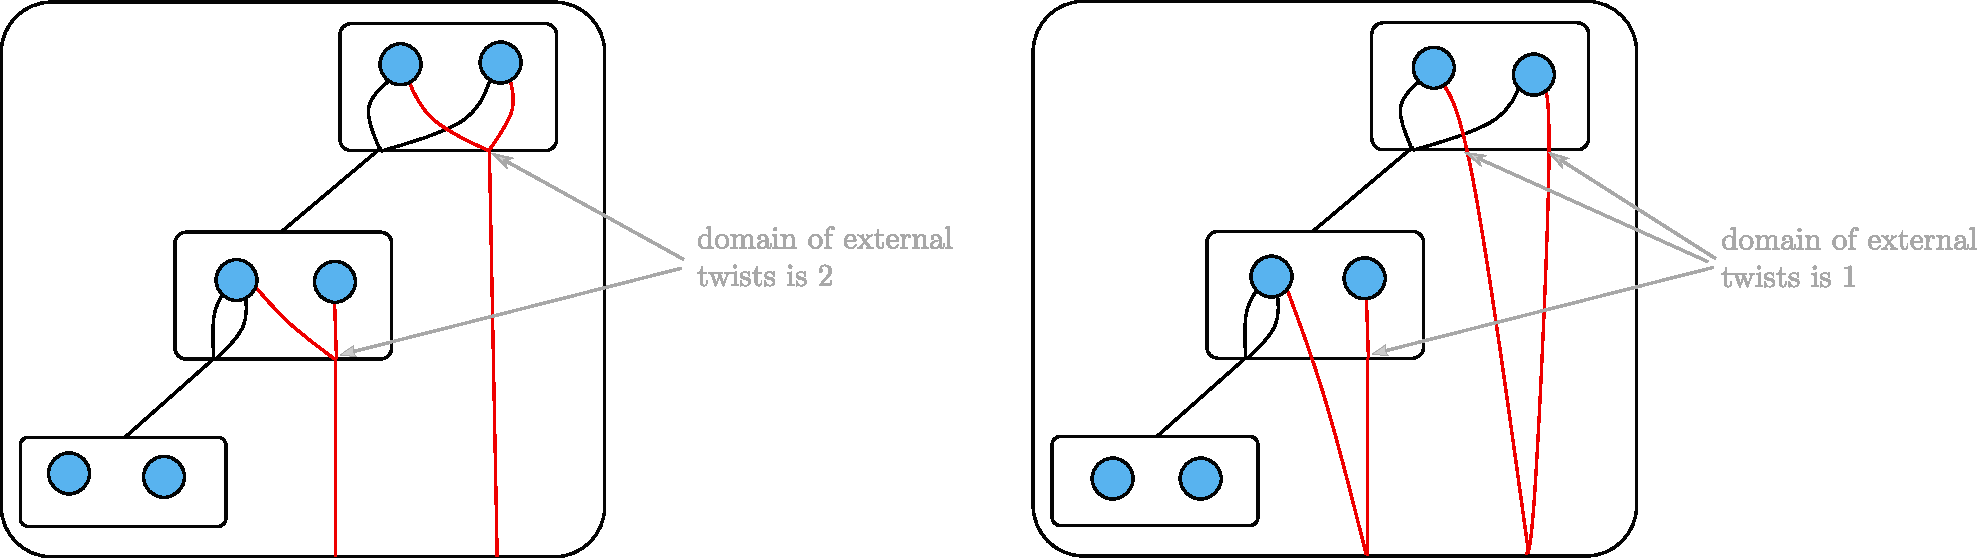
\includegraphics[scale=.4]{external-unfold.pdf}
\end{center}
\end{enumerate}

